\section{Introduzione generale}

\todo{Se volete yappare per allungarla fate pure}
\subsection{Statement}
Il sistema progettato vuole ricreare una applicazione desktop per il gioco del
Fantacalcio. I partecipanti al gioco sono in grado di creare, entrare e gestire le leghe e i 
propri fanta team: in particolare, sono in grado di schierare una formazione per la successiva partita
da giocare. Il sistema inoltre permette a varie testate giornalistiche di registrarsi e, 
una volta selezionate dall'admin della lega, di dare i voti ai calciatori.
\subsubsection{Actors}
Il sistema prevede tre tipi di utenti distinti, ciascuno con capacità diverse:
\begin{itemize}
    \item \textbf{FantaUser}: l'utente base dell'applicazione è in grado di entrare in leghe già esistenti per
    competere con gli altri giocatori schierando la formazione migliore in ogni giornata
    \item \textbf{Admin}: è un utente base che è anche admin di una lega. Si occupa di generare il calendario,  
    assegnare o rimuovere i calciatori dai team e di calcolare i risultati delle partite alla fine della giornata
    \item \textbf{Journalist}: è l'utente della lega che si occupa di assegnare i voti ai calciatori ad ogni giornata del campionato
\end{itemize}
\subsection{Requisiti Funzionali}
L'applicazione supporta le principali operazioni del gioco del fantacalcio, divise in base al ruolo
che l'utente ricopre nelle leghe in cui partecipa.
\begin{itemize}
    \item \textbf{Crea lega}: qualsiasi utente può creare una nuova lega, di cui diventa admin,
     per giocare con i propri amici.
    \item \textbf{Unirsi ad una lega come fanta manager}: qualsiasi utente può unirsi
    ad una lega a patto di conoscere il suo nome ed il suo codice. Una voltra dentro la
    lega l'utente potrà vederne i dettagli e potrà gestire il proprio team.
    \item \textbf{Unirsi alla lega come giornalista}: un utente può entrare in una lega non come manager
    ma come giornalista, il cui compito è quello di assegnare i voti ai calciatori.
    \item \textbf{Inserire la formazione}: prima di ogni giornata ogni utente che non è
    giornalista può schierare la propria formazione per quella giornata e lega.
    \item \textbf{Gestire la lega}: l'admin di una lega deve essere in grado di gestirla,
    ciò comporta l'assegnare i calciatori ai team, generare il calendario, calcolare i risultati
    delle partite e scandire l'avanzamento del gioco.
    \item \textbf{Assegnare voti ai calciatori}: gli utenti di tipo giornalista devono essere in grado di assegnare
    dei voti ai calciatori per la giornata in corso della lega in cui l'utente partecipa.
\end{itemize}

\subsection{Architettura}
\begin{figure}
    \centering
    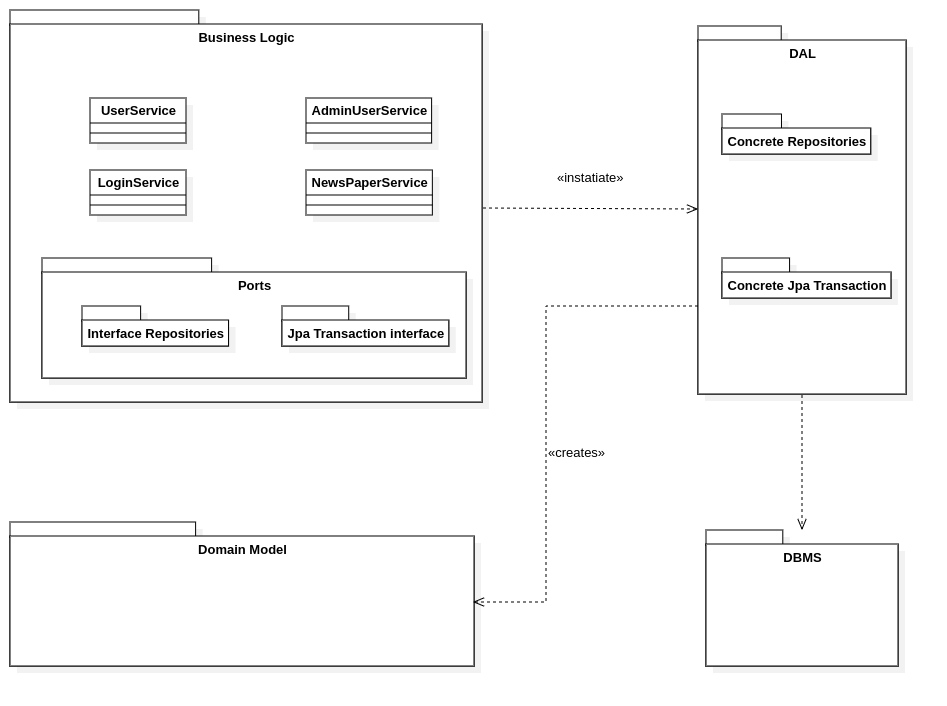
\includegraphics[width=0.8\textwidth]{Resources/graficiUML/Overview.png}        
    \caption{Overview dell'architettura.}
    \label{fig:overview dell'architettura}
\end{figure}
Il sistema è stato sviluppato in moduli ciascuno dei quali si occupa di compiti specifici.
Ciò permette di separare le responsabilità rendendo il codice più organizzato e semplice 
da manutenere e da estendere.
\begin{itemize}
    \item \textbf{Business Logic}: contiene le classi che si occupano della logica di 
    business. Tra queste ci sono i services che gestiscono le operazioni che i vari 
    attori sono i grado di compiere e i pacchetti che si occupano di gestire le transazioni con \textbf{JPA} e il pacchetto 
    che contiene le interfacce dei repository.
    \item \textbf{Domain Model}: contiene le entità annotate dell'applicazione
    \item \textbf{Repositories}: contiene le implementazione concreta dei repositories che si interfacciano con il database
\end{itemize}
In seguito ciascuno di questi pachhetti verrà analizzato in maniera più dettagliata.

\subsubsection{Dipendenze}
L'applicazione utilizza delle dipendenze esterne per la persistenza dei dati, 
per l'implementazione dei test e per la realizzazione dell'interfaccia grafica.

\begin{itemize}
    \item \textbf{JPA}: Java Persistence API, specifica standard che consente di gestire in maniera astratta la 
    persistenza dei dati su database relazionali, semplificando l'interazione con le entità tramite annotazioni 
    e query ad alto livello.
    
    \item \textbf{JUnit}: framework di testing unitario per Java che permette di automatizzare i test delle singole
     componenti, verificandone il corretto funzionamento e supportando l'integrazione nei processi di build.
    
    \item \textbf{Mockito}: libreria di supporto ai test che consente di creare oggetti fittizi (mock) per simulare 
    le dipendenze esterne e isolare le unità da testare, favorendo un approccio di testing modulare e controllato.
    
    \item \textbf{H2 Database}: database relazionale in-memory leggero e veloce, utilizzato durante lo sviluppo e il 
    testing per evitare la dipendenza da un database esterno, garantendo facilità di configurazione e rapidità di esecuzione.
    
    \item \textbf{Java Swing}: libreria grafica inclusa nel JDK per la realizzazione dell'interfaccia utente, 
    che fornisce componenti GUI (bottoni, menu, finestre, etc\dots) per costruire applicazioni desktop interattive.

    \todo{aggiungere dipendenze se mancano}
\end{itemize}

\subsection{Strumenti utilizzati}
Il codice è stato scritto in Java utilizzando \textbf{IntelliJ Idea} ed \textbf{Eclipse}.
La \textbf{GUI} è stata scritta utilizzando \textbf{Java Swing} e \textbf{Window Builder} \todo{Andre aggiungi la descrizione di cosa può fare}
Per la costruzione degli \textbf{UML} è stato utilizzato \textbf{StarUML} mentre per il versionamento
del codice è stato utilizzato \textbf{Github}. Inoltre sono stati usati vari \textbf{LLMS} come 
aiuto nella scrittura del codice, in particolare \textbf{Copilot}, \textbf{ChatGpt} e \textbf{Gemini}.